\section{Engineering a Real-life eHealth Service with HEADS}

This section describes how the HEADS approach has been applied to the TellU's eHealth system. 

\subsection{Overall Architecture}
The overall architecture of the eHealth system is depicted in Figure~\ref{fig:fig3}. The system is composed of a home gateway which runs on a Raspberry Pi 2 (1 GHz ARMv7, 1GB RAM, Linux). This gateway is connected to a number of field nodes (typically one per main room in the house) via WiFi. Field nodes run on an Intel Edison (400 MHz x86, 1GB RAM, WiFi and Bluetooth Low Energy (BLE)). Each field node has a pressure cell integrated in order to provide an accurate measurement of the pressure in each room. A wearable sensor node running on a low power resource-constrained ARM Cortex M3 (80 MHz, 256 KB RAM) also integrates a pressure cell and regularly broadcasts air pressure measurement to all field node that are in the BLE range (typically 10m indoor). Based on these pressure measurements and the intensity of the BLE signal, field node can determine the position of the person in the house and if the person has feel (by computing an air pressure differential between the person's sensor and the fixed pressure in the field node). In addition, a set of sensor nodes are deployed in different rooms to measure temperature and light. Those nodes run on an Arduino Yùn, which is composed of a resource-constrained microcontroller (16 MHz AVR-8bit, 2.5 KB RAM, no OS) and an embedded Linux processor (400 MHz MIPS, 64 MB RAM, WiFi, OpenWRT). The microcontroller part of the Yùn is used to interact with the physical temperature and light sensors while the MIPS CPU and its embedded WiFi is used to communicate with the Gateway. Finally, the gateway also integrates a Z-Wave radio chip that can control and interact with a set of devices (switches, etc). 

\begin{figure*}[!t]
	\centering
	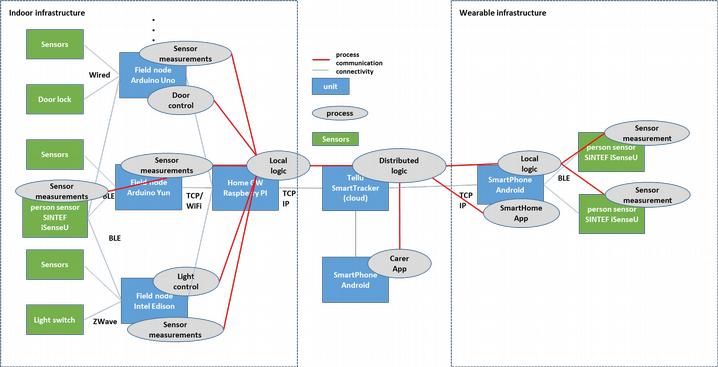
\includegraphics[width=0.7\linewidth]{figures/fig3}
	\caption{Safe@Home system architecture}
	\label{fig:fig3}
\end{figure*}



This particular HD-Service thus relies on an heterogeneous infrastructure composed from rather powerful 32-bit X86 and ARM processors with 1 GB RAM down to 8-bit AVR microcontroller running at 16 MHz (about 60 times slower) and embedding only 2.5 KB RAM (about 400 000 times less). It also integrates a variety of radio protocols such as WiFi, BlueTooth or Z-Wave. 

\subsection{Implementation of the Field Node}

At design/implementation time, the Field Node is composed of 8 core components implementing the logic of the node, and 2 other components that allows the field node to push information to the gateway via MQTT. Each of the implementation component is available as: 
\begin{itemize}
\item A Platform-Independent Component (PIC), which describes the interfaces of the component i.e., the port and messages it exposes. Some PICs can also provide a full implementation of their behavior, if this behavior does not imply using low-level libraries/drivers that directly interfaces with the hardware or system APIs. 
\item A Platform-Specific Component (PSC), which describes the full behavior of a component including the access to hardware drivers and system APIs. 
\end{itemize}

For example, the PIC associated to the BLE component describes messages related to the status of the BLE connection, such as stateChange (st : String); discover (peripheral : String); scanStart (); scanStop (). Those messages are orchestrated in the BLE PSC by a state machine (see Figure \ref{fig:fig4}) interfacing with the "noble" JavaScript module to deal with low-level details related to BlueTooth. 

\begin{figure}[t]
	\centering
	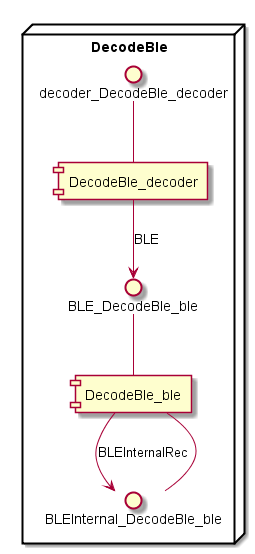
\includegraphics[width=0.25\linewidth]{figures/fig4}
	\caption{Component diagram of BLE and Decoder}
	\label{fig:fig4}
\end{figure}

Overall, the Field Node is implemented with ~300 LoC for the PICs and ~1100 LoC for the PSCs. It produces ~2000 LoC of JavaScript source code. This code can simply be run by executing the main.js file with Node.JS. However, this default implementation is rather monolithic at runtime and does not provide any dynamic reconfiguration capabilities. In order to provide such capabilities, this code is automatically wrapped into a component that can be manipulated and adapted at runtime. This additional component is fully generated and contained within 170 LoC. The automated wrapping is illustrated in Figure \ref{fig:fig5}. 

\begin{figure}[h]
	\centering
	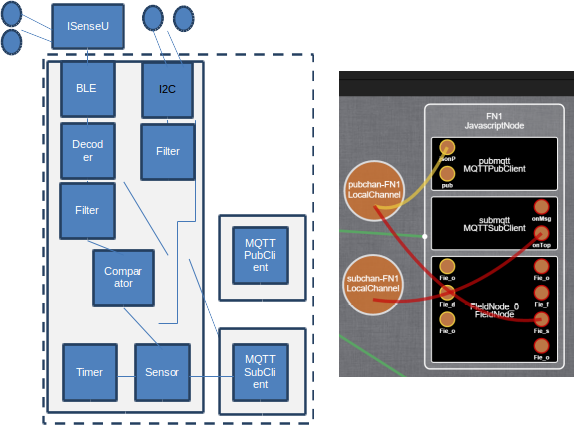
\includegraphics[width=0.75\linewidth]{figures/fig5-b}
	\caption{Field-Node component structure and actual Deployment}
	\label{fig:fig5}
\end{figure}


\subsection{Deployment and Operation of the Fall Detection service}
All the field node are described by 3 scripts. The first one is a root script basically describing the default configuration of the node, containing information about the network and how to connect to the rest of the system. It is shown in Figure~\ref{fig:fig6}

\begin{figure}[h]
	\centering
	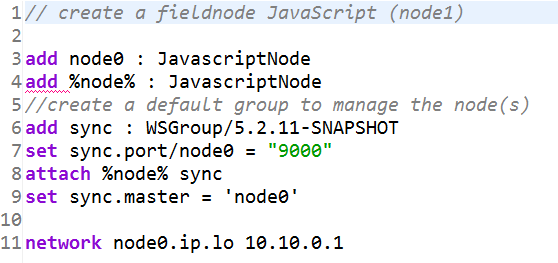
\includegraphics[width=0.6\linewidth]{figures/fig6}
	\caption{Default configuration of Field-Node}
	\label{fig:fig6}
\end{figure}

The second one is a script that will be executed whenever the field node connects to the network. This script adds a few components and connectors so that the field node can execute its logic and connect to the gateway via MQTT. This script is shown in Figure \ref{fig:fig7}. 
Finally, the third script simply remove the whole FieldNode from the model when the field node disappears from the network. Using those three scripts, the model and the running system are always in sync. Only field nodes that are actually connected to the network will appear in the model.% For example Figure \ref{fig:fig8} shows the configuration of the running system after two field nodes have connected. 

\begin{figure}[h]
	\centering
	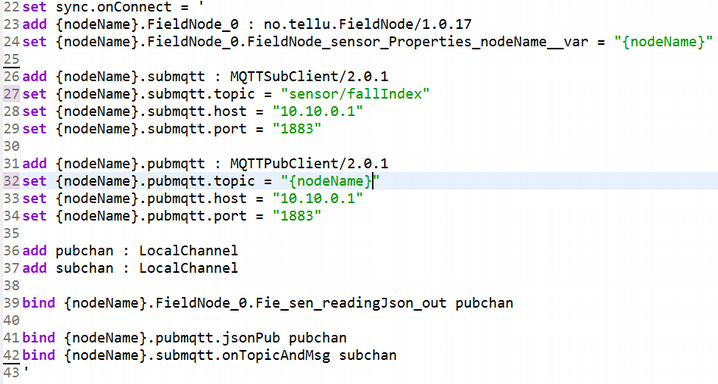
\includegraphics[width=1\linewidth]{figures/fig7}
	\caption{onConnect fragment of Home-GW inHEADS deployment model}
	\label{fig:fig7}
\end{figure}


%\begin{figure}[h]
%	\centering
%	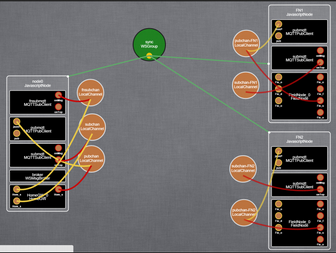
\includegraphics[width=1\linewidth]{figures/fig8}
%	\caption{onConnect fragment of Home-GW inHEADS deployment model}
%	\label{fig:fig8}
%\end{figure}

\subsection{Summary}
The eHealth service implemented by the TellU company involves are rather heterogeneous infrastructure composed of X86, ARM, MIPS and AVR nodes, ranging from 1GHz CPU with 1GB RAM down to 16MHz microcontroller with 2.5 KB RAM. All the code generated for this service (in JavaScript for the larger nodes and C for the smaller nodes) worked out of the box, without any manual modifications. All the libraries TellU needed to use (to interact with Z-Wave, BlueTooth, GPIO on the Intel Edison, etc or to communicate over MQTT) could be integrated with no major issues, either in the HEADS Modelling Language, or directly in the target language as a HEADS component.  

A few limitations were noted by TellU. Deploying code on resource-constrained devices can sometimes be cumbersome, as the generated code first needs to be cross-compiled and then uploaded to the device. This limitation could easily be addressed by extending the extension point related to build scripts so that it could also run the scripts using a command line the user can override. By default the C compiler would just run make. When compiling and uploading to Arduino it would execute: \texttt{avrdude -CD:avrdude.conf -v -v -v -v -patmega328p -carduino -P.COM22 -b57600 -D -Uflash:w:myProgram.cpp.hex:i}. 

Regarding the tooling, TellU was rather satisfied with the integration of the different languages and tools within the Eclipse IDE and simply noted some specific cases where code completion does not yet work on par with e.g. Java code completion. Other than that, the languages and tools are usable.

\subsection{Lessons learned}
Several developers at TellU, well acquainted with Java, were able to rapidly get started with the concepts and tools described in this approach. A series of tutorials covering the different concepts, and including exercises to be completed by the participants, was completed within a couple of days~\footnote{https://github.com/HEADS-project/training}. Before implementing the eHealth service, TellU developers have been working on the past few years on the backend service, collecting data and performing analytics. Integrating directly with sensors and gateways was thus a new activity. Most of the learning curve was related to learning how to interact directly with hardware. The HEADS approach actually speed up the process by allowing integrating with C and JavaScript libraries (not popular languages at TellU) without writing advanced C and JavaScript, as most of the logic could be expressed in a platform independent way. In particular, our generative and modular component-based approach for heterogeneous and distributed system allowed and efficient co-development and continuous evolution of this eHealth service. Once interfaces have been defined, it was easy for TellU to define mockups for the components that were not yet implemented and still be able to run the whole system. Mockups were replaced in an iterative way.

Regarding the integration with new languages and platforms, most of the compilers (POSIX C for Linux, Java and JavaScript) have been developed by people heavily involved in the definition of the HEADS Design Language and the Transformation Framework. It is thus hard to conclude on how difficult it is to implement a completely new compiler, other than it took 3000 LoC for Java and JavaScript and about 7000 LoC for POSIX C, which is far way less than writing a ``real'' compiler (GCC being 14 millions LoC). An experiment conducted with another department at SINTEF with people not involved in the development of the language and framework showed it is possible to extend the C compiler to support another ``dialect'' for ARM microcontrollers. This took about 2000 LoC and a couple of weeks for the embedded C expert (with only basic Java knowledge) to get this compiler fully functional. While the time to write this compiler could have been reduced e.g. with better documentation, the two weeks spend here were almost entirely saved by developers at TellU who could just get started with this new platform without building a detailed knowledge of C development on this platform.